%% ============================================================
%%  V. Peilivanidis — ARPA Hellenic Logical Systems
%% ============================================================
\pdfoutput=1
\documentclass[11pt,a4paper]{article}

%% --- Font stack  ---
\usepackage[T1]{fontenc}
\usepackage[utf8]{inputenc}
\usepackage{amsmath, amssymb, amsthm}
\usepackage{newpxtext, newpxmath}
\usepackage[scaled=0.88]{inconsolata}
\usepackage{microtype}

%% --- Page geometry ---
\usepackage[a4paper, left=3.0cm, right=3.0cm, top=3.2cm, bottom=3.2cm]{geometry}

%% --- Color palette ---
\usepackage{xcolor}
\definecolor{accent}{HTML}{1F4E8C}
\definecolor{coderule}{HTML}{C8D8EE}
\definecolor{codebg}{HTML}{F4F7FC}
\definecolor{boxbg}{HTML}{EDF2FA}
\definecolor{boxrule}{HTML}{1F4E8C}
\definecolor{graytext}{HTML}{555555}
\definecolor{lightrule}{HTML}{CCCCCC}

%% --- Hyperlinks ---
\usepackage[colorlinks=true, citecolor=accent, linkcolor=accent,
            urlcolor=accent, breaklinks=true]{hyperref}
\usepackage{url}

%% --- Math ---
\usepackage{bm}

%% --- Graphics ---
\usepackage{graphicx}
\usepackage{booktabs}
\usepackage{tabularx}
\usepackage{float}

%% --- TikZ + PGFPlots ---
\usepackage{tikz}
\usetikzlibrary{arrows.meta, shapes.geometric, shapes.misc,
                positioning, calc, fit, backgrounds}
\usepackage{pgfplots}
\pgfplotsset{compat=1.18}

%% --- Captions ---
\usepackage[
  font={small, color=graytext},
  labelfont={bf, color=black},
  labelsep=period,
  justification=justified,
  singlelinecheck=false
]{caption}

%% --- Section titles ---
\usepackage{titlesec}
\titleformat{\section}
  {\normalfont\large\bfseries}{\thesection}{0.7em}{}
  [\vspace{2pt}{\color{accent}\hrule height 0.5pt}\vspace{2pt}]
\titleformat{\subsection}
  {\normalfont\normalsize\bfseries}{\thesubsection}{0.7em}{}
\titleformat{\subsubsection}
  {\normalfont\normalsize\itshape}{\thesubsubsection}{0.7em}{}
\titlespacing{\section}{0pt}{14pt plus 4pt minus 2pt}{6pt plus 2pt}
\titlespacing{\subsection}{0pt}{10pt plus 3pt minus 1pt}{4pt plus 1pt}

%% --- Header / footer ---
\usepackage{fancyhdr}
\pagestyle{fancy}
\fancyhf{}
\fancyhead[L]{\small\color{graytext}R. Peili}
\fancyhead[R]{\small\color{graytext}Learning Phase Angles for QSP via Gradient Descent}
\fancyfoot[C]{\small\thepage}
\renewcommand{\headrulewidth}{0.3pt}
\renewcommand{\footrulewidth}{0pt}

\fancypagestyle{firstpage}{
  \fancyhf{}
  \fancyfoot[C]{\small\thepage}
  \renewcommand{\headrulewidth}{0pt}
  \renewcommand{\footrulewidth}{0pt}
}

%% --- Contribution box ---
\usepackage{tcolorbox}
\tcbuselibrary{skins, breakable}
\tcbset{
  contribbox/.style={
    enhanced, breakable,
    colback=boxbg, colframe=accent,
    leftrule=3pt, toprule=0.4pt, bottomrule=0.4pt, rightrule=0.4pt,
    arc=2pt, outer arc=2pt,
    left=8pt, right=8pt, top=6pt, bottom=6pt,
    fonttitle=\small\bfseries\color{accent},
    title={Summary of Contributions},
    attach boxed title to top left={yshift=-2mm, xshift=6pt},
    boxed title style={colback=white, colframe=white}
  }
}

%% --- Code listings ---
\usepackage{listings}
\lstdefinestyle{qspcode}{
  language=Python,
  basicstyle=\small\ttfamily,
  keywordstyle=\color{accent}\bfseries,
  stringstyle=\color{graytext},
  commentstyle=\color{graytext}\itshape,
  backgroundcolor=\color{codebg},
  frame=single,
  rulecolor=\color{coderule},
  framexleftmargin=4pt,
  xleftmargin=4pt,
  xrightmargin=2pt,
  numbers=left,
  numberstyle=\tiny\color{graytext},
  numbersep=8pt,
  breaklines=true,
  showstringspaces=false,
  tabsize=4,
  aboveskip=8pt, belowskip=6pt
}
\lstset{style=qspcode}

%% --- Bibliography ---
\usepackage[style=numeric-comp, backend=biber,
            sortcites=true, giveninits=true,
            maxcitenames=2, maxbibnames=99,
            doi=true, url=false, isbn=false]{biblatex}
\addbibresource{references.bib}

%% --- Line spacing ---
\setlength{\parskip}{4pt}
\setlength{\parindent}{1em}

%% ============================================================
%%  METADATA
%% ============================================================
\title{%
  \vspace{-0.5cm}%
  {\LARGE\bfseries Learning Phase Angles for Quantum Signal Processing%
  \\ via Gradient Descent}\\[0.55em]
  {\normalsize\normalfont\color{accent}
   A Differentiable Circuit Approach — Reference Implementation with JAX and PennyLane}
}

\author{%
  \textbf{Ross Peili (Vladimiros Peilivanidis)}\\[0.25em]
  {\small ARPA Hellenic Logical Systems, Thessaloniki, Greece}\\
  {\small \href{mailto:vpeilivanidis@gmail.com}{\texttt{vpeilivanidis@gmail.com}}}
  \quad{\small ORCID: \href{https://orcid.org/0009-0003-0121-465X}{0009-0003-0121-465X}}
}

\date{%
  \small Draft, June 2026\quad|\quad
  {\normalfont\color{graytext}%
   Code: \href{https://github.com/rosspeili/trainable-qsp-angles}{\texttt{github.com/rosspeili/trainable-qsp-angles}}
   \quad|\quad
   Notebook: \texttt{demo.ipynb}}%
}

\begin{document}

\maketitle
\thispagestyle{firstpage}

%% Abstract environment
\begin{center}
\begin{minipage}{0.92\textwidth}
\small
\textbf{Abstract.}\quad
Quantum Signal Processing (QSP) is a foundational algorithmic primitive that encodes polynomial transformations of a scalar signal into a single-qubit quantum circuit via a structured sequence of phase-shifted oracle calls. The canonical approach computes phase angles analytically from a target polynomial --- a well-studied but numerically sensitive problem. We present an empirical study of \emph{learning} QSP phase angles from random initialization using gradient-based optimization on a JAX-traceable \emph{flat} circuit---independent of any particular quantum SDK, though we report a reference implementation in PennyLane. This route is useful when analytic solvers are unavailable or embedded in a larger differentiable pipeline. We train a degree-5 circuit to approximate a Chebyshev expansion of $\sin(x)$ via Adam, reaching a mean squared error of $4.82 \times 10^{-4}$ within 500 steps (single-seed benchmark; multi-seed statistics in the accompanying code). We identify and document a non-obvious incompatibility between high-level QSVT template APIs (exemplified by PennyLane's \texttt{qml.QSVT}) and JAX tracing, and provide a flat-circuit pattern that preserves end-to-end differentiability across frameworks. Code, experiment scripts, and an interactive notebook are publicly available under the Apache~2.0 license.

\vspace{6pt}
\noindent\textbf{Keywords:}\quad
quantum signal processing (QSP) $\cdot$
quantum singular value transformation (QSVT) $\cdot$
phase angle optimization $\cdot$
differentiable quantum circuits $\cdot$
gradient descent $\cdot$
Chebyshev polynomial approximation $\cdot$
automatic differentiation $\cdot$
JAX $\cdot$
differentiable quantum programming
\end{minipage}
\end{center}

\vspace{0.5em}
\noindent\rule{\textwidth}{0.3pt}
\vspace{0.3em}

%% ============================================================
\section{Introduction}
%% ============================================================

The history of quantum algorithms is, in large part, a history of discovering that quantum mechanics permits a surprisingly rich set of mathematical operations to be performed efficiently on physical hardware. Among the most elegant of such discoveries is \emph{Quantum Signal Processing} (QSP) --- a framework establishing a precise and complete characterization of the polynomial transformations achievable by a single-qubit quantum circuit interleaved with repeated queries to a signal oracle~\cite{low2017optimal}.

The core insight of QSP is deceptively simple. Given a scalar signal $x \in [-1, 1]$ encoded in the matrix elements of a unitary oracle $W(x)$, a circuit that alternates between calls to $W(x)$ and single-qubit $Z$-rotations (the \emph{phase angles}) encodes a polynomial in $x$ in the expectation value of the final state. The converse is equally powerful: for any real polynomial satisfying mild bounded-norm and parity conditions, there exist phase angles that realize it exactly. This completeness result~\cite{low2017optimal, gilyen2019quantum} elevates QSP to the status of a \emph{universal language} for quantum algorithms.

The implications are substantial. Algorithms for Hamiltonian simulation, quantum linear systems, amplitude amplification, quantum phase estimation, and ground-state preparation can all be expressed as instances of QSP or its multi-qubit generalization, Quantum Singular Value Transformation (QSVT)~\cite{martyn2021grand, gilyen2019quantum}. This ``grand unification'' perspective reveals that many apparently unrelated quantum algorithms are in fact the same circuit architecture with different phase angle sequences --- turning quantum algorithm design into a problem of polynomial approximation.

\subsection{The Phase Angle Problem}

The practical challenge is computing those phase angles. Given a target polynomial $P(x)$, classical algorithms exist to recover the exact phase angles $(\phi_0, \phi_1, \ldots, \phi_d)$. However, these analytic solvers are numerically fragile at high polynomial degree~\cite{haah2019product, chao2020finding}, and they require the target polynomial to be known in closed form --- an assumption that breaks down in variational settings where the target is implicitly defined by a downstream loss function.

\subsection{This Work}

We explore a complementary approach: \emph{learning} phase angles from random initialization using gradient descent. The key observation is that a QSP circuit, when implemented correctly as a differentiable quantum program, admits automatic differentiation through all its parameters. This makes it possible to minimize any differentiable loss over the phase angles using standard optimizers.

We demonstrate this via a publicly available reference implementation~\cite{peili_trainable_qsp_2026} using PennyLane~\cite{pennylane2022} with JAX~\cite{jax2018github}; the underlying flat-circuit recipe transfers to other SDKs such as Qiskit~\cite{qiskit2024}, Cirq~\cite{cirq2024}, or TensorFlow Quantum~\cite{broughton2020tfq} when parameters remain live in the autodiff graph. We identify and resolve a non-obvious incompatibility between template-based QSVT constructors and JAX tracing in our PennyLane code path, and provide the correct flat-circuit pattern.

\begin{tcolorbox}[contribbox]
\begin{itemize}\setlength\itemsep{3pt}
  \item[\textbf{C1.}] We show that high-level QSVT template APIs can capture operator values at circuit-build time, breaking JAX differentiability through phase angles (observed in PennyLane's \texttt{qml.QSVT}), and provide a flat-circuit workaround that preserves end-to-end gradient flow.
  \item[\textbf{C2.}] We provide a reproducible degree-5 benchmark (Chebyshev $\sin$ target) with experiment scripts, reporting convergence from MSE $\approx 1.44$ to $4.82\times10^{-4}$ in 500 Adam steps for the reference seed.
  \item[\textbf{C3.}] We provide a practical decision guide for when gradient training is preferable to analytic angle computation.
  \item[\textbf{C4.}] All code, experiments, and an interactive notebook are released under the Apache~2.0 license at \href{https://github.com/rosspeili/trainable-qsp-angles}{\texttt{github.com/rosspeili/trainable-qsp-angles}}.
\end{itemize}
\end{tcolorbox}

%% ============================================================
\section{Background: Quantum Signal Processing}
%% ============================================================

\subsection{Signal Oracle}

The standard QSP signal oracle $W(x)$ encodes a scalar $x \in (-1,1)$ in its matrix elements:
\begin{equation}
  W(x) \;=\; H\,R_Z(-2\arccos x)\,H
  \;=\;
  \begin{pmatrix} x & i\sqrt{1-x^2} \\ i\sqrt{1-x^2} & x \end{pmatrix},
\end{equation}
where $H$ is the Hadamard gate and $R_Z(\theta)=e^{-i\theta Z/2}$. The signal $x$ appears in the top-left matrix element, accessible as a quantum amplitude. Geometrically, $W(x)$ rotates the Bloch sphere state by angle $\theta = 2\arccos(x)$ around the $x$-axis, mapping $|0\rangle$ to $x|0\rangle + i\sqrt{1-x^2}|1\rangle$ (Figure~\ref{fig:bloch}).

\begin{figure}[ht]
\centering
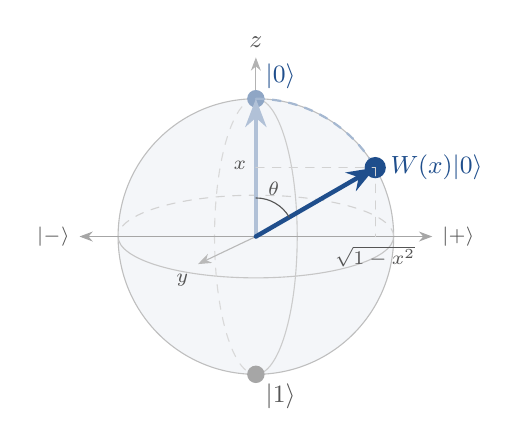
\begin{tikzpicture}[scale=1.75, >=Stealth, line cap=round]

  \fill[accent!5] (0,0) circle (1);
  \draw[gray!50, thin] (0,0) circle (1);

  \draw[dashed, gray!35, thin] (1,0) arc (0:180:1 and 0.30);
  \draw[gray!45, thin] (-1,0) arc (180:360:1 and 0.30);

  \draw[dashed, gray!30, thin] (0,1) arc (90:270:0.30 and 1);
  \draw[gray!40, thin] (0,-1) arc (270:450:0.30 and 1);

  \draw[->, thin, gray!70] (0,0,0) -- (1.28,0) node[right, font=\scriptsize, graytext] {$|{+}\rangle$};
  \draw[->, thin, gray!70] (0,0,0) -- (-1.28,0) node[left, font=\scriptsize, graytext] {$|{-}\rangle$};
  \draw[->, thin, gray!55] (0,0) -- (-0.42,-0.20) node[below left, font=\scriptsize, graytext] {$y$};
  \draw[->, thin, gray!60] (0,0) -- (0, 1.30) node[above, font=\small, graytext] {$z$};

  \fill[accent!50] (0,1) circle (1.8pt);
  \node[above right, font=\small\bfseries, accent] at (0,1) {$|0\rangle$};
  \fill[gray!70] (0,-1) circle (1.8pt);
  \node[below right, font=\small, graytext] at (0,-1) {$|1\rangle$};

  \draw[accent!40, dashed, thick] (0,1) arc (90:30:1);

  \draw[->, ultra thick, accent!35] (0,0) -- (0,1);

  \draw[->, ultra thick, accent] (0,0) -- ({sin(60)},{cos(60)});
  \fill[accent] ({sin(60)},{cos(60)}) circle (2.2pt);
  \node[right, font=\small\bfseries, accent] at ({sin(60)+0.04},{cos(60)})
    {$W(x)|0\rangle$};

  \draw[thin, graytext] (0,0.28) arc (90:30:0.28);
  \node[font=\scriptsize, graytext] at (0.13, 0.35) {$\theta$};

  \draw[thin, dashed, gray!35] ({sin(60)},{cos(60)}) -- ({sin(60)},0)
    node[below, font=\scriptsize, graytext] {$\sqrt{1-x^2}$};
  \draw[thin, dashed, gray!35] (0,{cos(60)}) -- ({sin(60)},{cos(60)});
  \node[left, font=\scriptsize, graytext] at (0,{cos(60)+0.02}) {$x$};

\end{tikzpicture}
\caption{Bloch sphere representation of the QSP signal oracle $W(x)$. The oracle rotates the initial state $|0\rangle$ (faint arrow) by angle $\theta = 2\arccos(x)$ around the $x$-axis, producing the state $W(x)|0\rangle = x|0\rangle + i\sqrt{1-x^2}|1\rangle$ (solid arrow). The signal $x$ appears as the $z$-projection (amplitude on $|0\rangle$), and $\sqrt{1-x^2}$ as the transverse component.}
\label{fig:bloch}
\end{figure}

\subsection{The QSP Sequence}


A degree-$d$ QSP circuit interleaves $d$ oracle calls with $d+1$ phase rotations $\boldsymbol{\phi}=(\phi_0,\ldots,\phi_d)\in\mathbb{R}^{d+1}$:
\begin{equation}
  U_{\mathrm{QSP}}(x;\boldsymbol{\phi})
  \;=\; R_Z(-2\phi_0)\prod_{k=1}^{d} W(x)\,R_Z(-2\phi_k).
\end{equation}
The expectation value $\langle X\rangle = \langle 0|U^\dagger X\,U|0\rangle$ is a degree-$d$ polynomial in $x$ determined entirely by $\boldsymbol{\phi}$.

\begin{figure}[ht]
\centering
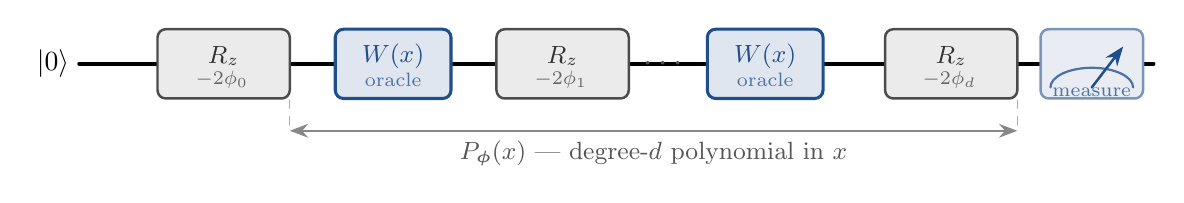
\begin{tikzpicture}[>=Stealth, x=1.05cm, y=1cm, line cap=round]

  \def\W{0.80}
  \def\H{0.44}

  \draw[line width=1.2pt] (-0.9,0) -- (12.1,0);

  \node[left, font=\normalsize\bfseries] at (-0.9,0) {$|0\rangle$};

  \foreach \cx/\lbl/\sub in {
    0.85/{$R_z$}/{$\!-2\phi_0$},
    4.95/{$R_z$}/{$\!-2\phi_1$},
    9.65/{$R_z$}/{$\!-2\phi_d$}}
  {
    \fill[black!8, draw=black!70, rounded corners=3pt, line width=0.9pt]
      (\cx-\W, -\H) rectangle (\cx+\W, \H);
    \node[font=\small\bfseries, text=black!80] at (\cx, 0.10) {\lbl};
    \node[font=\scriptsize, text=black!60] at (\cx,-0.20) {\sub};
  }

  \foreach \cx in {2.90, 7.40} {
    \fill[accent!14, draw=accent, rounded corners=3pt, line width=1.1pt]
      (\cx-0.70,-\H) rectangle (\cx+0.70,\H);
    \node[font=\small\bfseries, text=accent] at (\cx, 0.10) {$W(x)$};
    \node[font=\scriptsize, text=accent!80] at (\cx,-0.20) {oracle};
  }

  \node[font=\large, text=graytext] at (6.20, 0) {$\cdots$};

  \begin{scope}[shift={(11.35,0)}]
    \fill[accent!10, draw=accent!60, rounded corners=3pt, line width=0.9pt]
      (-0.62,-\H) rectangle (0.62,\H);
    \draw[accent!80, line width=0.8pt]
      (-0.50,-0.30) arc (180:0:0.50 and 0.25);
    \draw[->, accent, line width=0.9pt]
      (0,-0.30) -- (0.38, 0.22);
    \node[font=\scriptsize, text=accent!80] at (0, -0.36) {measure};
  \end{scope}

  \draw[<->, thick, graytext!70] (1.65,-0.85) -- (10.45,-0.85)
    node[midway, below, font=\small, text=graytext]
    {$P_{\boldsymbol{\phi}}(x)$ — degree-$d$ polynomial in $x$};
  \draw[dashed, graytext!50, thin] (1.65,-0.46) -- (1.65,-0.85);
  \draw[dashed, graytext!50, thin] (10.45,-0.46) -- (10.45,-0.85);

\end{tikzpicture}
\caption{QSP circuit for degree $d$. Gray boxes are trainable phase rotations $R_z(-2\phi_k)$; blue boxes are signal oracle calls $W(x)$. The final measurement yields the expectation value $\langle X\rangle = P_{\boldsymbol{\phi}}(x)$, a degree-$d$ polynomial in $x$ fully determined by the phase angle sequence $\boldsymbol{\phi}$.}
\label{fig:qsp_circuit}
\end{figure}


\subsection{Completeness Theorem}

The central result of QSP theory~\cite{low2017optimal, martyn2021grand} establishes a bijection between phase sequences and polynomials:

\begin{quote}\itshape
For any real polynomial $P$ of degree $d$ satisfying (i) $|P(x)|\le 1$ for all $x\in[-1,1]$, and (ii) $P$ has definite parity, there exist $(\phi_0,\ldots,\phi_d)\in\mathbb{R}^{d+1}$ such that $\langle X\rangle = P(x)$ for all $x\in(-1,1)$.
\end{quote}

The QSVT generalization~\cite{gilyen2019quantum} extends this to matrix-valued signals, enabling block-encoded polynomial transformations of arbitrary Hermitian operators. Table~\ref{tab:algorithms} lists representative quantum algorithms expressible as QSP instances.

\begin{table}[ht]
\centering
\small
\begin{tabularx}{\textwidth}{@{} l X l @{}}
  \toprule
  \textbf{Algorithm} & \textbf{Target polynomial} & \textbf{Reference} \\
  \midrule
  Hamiltonian simulation    & $e^{-iHt}$ (Jacobi-Anger expansion)   & \cite{low2019hamiltonian} \\
  Amplitude amplification   & Step-function approximation            & \cite{martyn2021grand} \\
  Quantum phase estimation  & Chebyshev spectral filter              & \cite{martyn2021grand} \\
  Ground-state preparation  & Low-pass spectral filter               & \cite{dong2021efficient} \\
  Quantum chemistry         & Matrix inversion ${\sim}1/x$           & \cite{babbush2018encoding} \\
  \bottomrule
\end{tabularx}
\caption{Quantum algorithms expressible as QSP instances. Each algorithm corresponds to a target polynomial; the phase angles provide the circuit that implements it.}
\label{tab:algorithms}
\end{table}

%% ============================================================
\section{Methods: Gradient-Based Phase Angle Learning}
%% ============================================================

\subsection{Optimization Objective}

Given a target polynomial $P_{\mathrm{target}}(x)$ satisfying QSP admissibility conditions, we minimize the mean squared error over a discrete signal grid $\{x_i\}_{i=1}^N \subset (-1,1)$:
\begin{equation}
  \boldsymbol{\phi}^* = \arg\min_{\boldsymbol{\phi}}\;\mathcal{L}(\boldsymbol{\phi})
  = \frac{1}{N}\sum_{i=1}^{N}\bigl(\langle X\rangle_{\boldsymbol{\phi}}(x_i) - P_{\mathrm{target}}(x_i)\bigr)^2.
  \label{eq:loss}
\end{equation}
Figure~\ref{fig:pipeline} illustrates the full training pipeline.

\begin{figure}[ht]
\centering
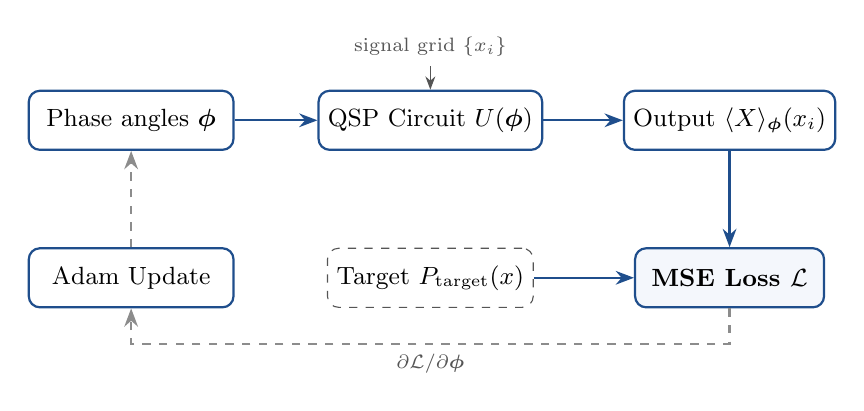
\begin{tikzpicture}[>=Stealth,
  box/.style={draw=accent, rounded corners=4pt, fill=white, thick,
              minimum width=2.6cm, minimum height=0.75cm,
              font=\small, align=center},
  lossbox/.style={draw=accent, rounded corners=4pt, fill=codebg, thick,
                  minimum width=2.4cm, minimum height=0.75cm,
                  font=\small\bfseries, align=center},
  tgtbox/.style={draw=graytext, dashed, rounded corners=4pt, fill=white,
                 minimum width=2.4cm, minimum height=0.75cm,
                 font=\small, align=center},
  fwd/.style={-Stealth, thick, accent},
  bwd/.style={-Stealth, thick, black!45, dashed},
  garr/.style={-Stealth, thin, graytext},
  lbl/.style={font=\scriptsize, text=graytext}
]

  \node[box]     (phases)  at (0,    0)   {Phase angles $\boldsymbol{\phi}$};
  \node[box]     (circuit) at (3.8,  0)   {QSP Circuit $U(\boldsymbol{\phi})$};
  \node[box]     (output)  at (7.6,  0)   {Output $\langle X\rangle_{\boldsymbol{\phi}}(x_i)$};

  \node[box]     (adam)    at (0,   -2.0) {Adam Update};
  \node[tgtbox]  (target)  at (3.8, -2.0) {Target $P_{\mathrm{target}}(x)$};
  \node[lossbox] (loss)    at (7.6, -2.0) {MSE Loss $\mathcal{L}$};

  \node[above=0.3cm of circuit, lbl] (sig) {signal grid $\{x_i\}$};

  \draw[fwd]  (phases)  -- (circuit);
  \draw[fwd]  (circuit) -- (output);
  \draw[garr] (sig)     -- (circuit);

  \draw[fwd]  (output)  -- (loss);
  \draw[fwd]  (target)  -- (loss);

  \coordinate (lb) at ([yshift=-0.45cm]loss.south);
  \coordinate (ab) at ([yshift=-0.45cm]adam.south);
  \draw[bwd] (loss.south) -- (lb) --
    node[below, lbl]{$\partial\mathcal{L}/\partial\boldsymbol{\phi}$}
    (ab) -- (adam.south);

  \draw[bwd] (adam.north) -- (phases.south);

\end{tikzpicture}
\caption{Gradient training pipeline. \textbf{Forward pass} (solid): phase angles $\boldsymbol{\phi}$ and signal grid $\{x_i\}$ enter the QSP circuit; the output is compared against the target polynomial in the MSE loss. \textbf{Backward pass} (dashed): gradients $\partial\mathcal{L}/\partial\boldsymbol{\phi}$ propagate via Adam to update $\boldsymbol{\phi}$.}
\label{fig:pipeline}
\end{figure}


\subsection{Target Polynomial}

The target is a degree-5 Chebyshev expansion of $\sin(x)$ using odd polynomials $T_k$ of the first kind:
\begin{equation}
  P_{\mathrm{target}}(x) = c_1 T_1(x) + c_3 T_3(x) + c_5 T_5(x),
\end{equation}
with $c_1=0.9775$, $c_3=-0.1564$, $c_5=0.0158$. This polynomial is odd, bounded in $[-1,1]$, and satisfies the QSP parity condition. Maximum deviation from $\sin(x)$ is $0.1738$ --- a degree-5 truncation artifact, not a QSP limitation.

\subsection{Circuit Implementation and the JAX Traceability Constraint}

High-level QSVT template constructors---including PennyLane's \texttt{qml.QSVT}---can build operator objects at circuit definition time, capturing concrete numerical values that exit JAX's abstract trace and produce zero gradients through the phase angles. The fix is a \emph{flat circuit} of primitive gates, keeping phase angles as live JAX arrays throughout. The same principle applies in other frameworks whenever templates materialize parameters before autodiff sees them.

\begin{lstlisting}[caption={Reference flat-circuit QSP implementation (PennyLane + JAX). The structure is portable; only the gate API differs in Qiskit, Cirq, or TFQ.}, label={lst:circuit}]
import pennylane as qp

@qp.qnode(dev, interface="jax", diff_method="backprop")
def qsp_qnode(phases, x):
    qp.RZ(-2.0 * phases[0], wires=0)
    for k in range(1, len(phases)):
        qp.Hadamard(wires=0)
        qp.RZ(-2.0 * jnp.arccos(x), wires=0)
        qp.Hadamard(wires=0)
        qp.RZ(-2.0 * phases[k], wires=0)
    return qp.expval(qp.PauliX(0))
\end{lstlisting}

\subsection{Technology Stack and Training Protocol}

\begin{table}[ht]
\centering\small
\begin{tabularx}{\textwidth}{@{} l l X @{}}
  \toprule
  \textbf{Component} & \textbf{Tool} & \textbf{Role} \\
  \midrule
  Quantum simulation (reference) & PennyLane 0.44+   & Differentiable QNode frontend; plugins available for Qiskit/Cirq/others \\
  Analytic baseline (optional)   & \texttt{poly\_to\_angles} & Convenience wrapper; Chao et al.\ solver usable independently \\
  Automatic diff.     & JAX 0.4.25+ (x64) & Gradient computation and JIT compilation \\
  Optimization        & Optax (Adam)       & Parameter updates, lr~$=0.05$, 500 steps \\
  Vectorization       & \texttt{jax.vmap} & Parallel evaluation over the signal grid \\
  Precision           & float64            & Numerical stability of $\arccos$ near $\pm 1$ \\
  \bottomrule
\end{tabularx}
\caption{Technology stack for the reference implementation. PennyLane is not mandatory for the method; see repository documentation for alternative SDKs.}
\label{tab:stack}
\end{table}

Phase angles are initialized uniformly in $[-0.5,0.5]$. A uniform grid of 64 signal points on $[-0.95,0.95]$ is used; the loss and gradient step are JIT-compiled, and circuit evaluations are batched via \texttt{jax.vmap}.

%% ============================================================
\section{Results}
%% ============================================================

\subsection{Convergence}

Starting from a random initialization with loss $\approx 1.44$, the Adam optimizer reduces the MSE by three orders of magnitude within the first 100 steps. By step 500, the learned phase angles are:
\begin{equation}
  \boldsymbol{\phi}^* \approx (-0.0733,\ -0.2631,\ -0.9651,\ 1.4105,\ 0.8982,\ -0.1731),
\end{equation}
yielding a final MSE of $4.82\times10^{-4}$ and a maximum pointwise error of $9.83\times10^{-2}$ against $P_{\mathrm{target}}$.

\begin{figure}[ht]
\centering
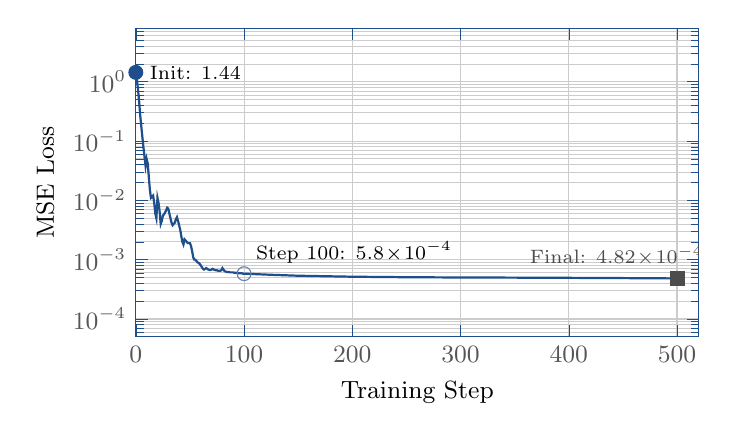
\begin{tikzpicture}
\begin{semilogyaxis}[
  width=0.72\textwidth, height=5.5cm,
  xlabel={Training Step},
  ylabel={MSE Loss},
  xmin=0, xmax=520,
  ymin=5e-5, ymax=8,
  xtick={0,100,200,300,400,500},
  grid=both,
  grid style={line width=0.3pt, draw=lightrule},
  major grid style={line width=0.4pt, draw=lightrule},
  axis line style={accent},
  tick style={accent},
  xlabel style={font=\small},
  ylabel style={font=\small},
  tick label style={font=\small, color=graytext},
  legend style={font=\small, at={(0.98,0.95)}, anchor=north east,
                draw=lightrule, fill=white},
]
\addplot[accent, thick] coordinates {
  (0,1.44) (1,1.10) (2,0.75) (3,0.48) (4,0.28)
  (5,0.18) (6,0.12) (7,0.080) (8,0.055) (9,0.038)
  (10,0.050) (11,0.042) (12,0.025) (13,0.015) (14,0.011)
  (15,0.0115) (16,0.0120) (17,0.0090) (18,0.0060) (19,0.0050)
  (20,0.0110) (21,0.0090) (22,0.0065) (23,0.0040) (24,0.0045)
  (25,0.0055) (26,0.0058) (27,0.0062) (28,0.0068) (29,0.0075)
  (30,0.0072) (31,0.0060) (32,0.0050) (33,0.0042) (34,0.0038)
  (35,0.0040) (36,0.0042) (37,0.0048) (38,0.0052) (39,0.0045)
  (40,0.0038) (41,0.0032) (42,0.0025) (43,0.0020) (44,0.0018)
  (45,0.0022) (46,0.0021) (47,0.0020) (48,0.0019) (49,0.0019)
  (50,0.0019) (51,0.0017) (52,0.0014) (53,0.0011) (54,0.0010)
  (55,0.0010) (56,0.00095) (57,0.00090) (58,0.00088) (59,0.00085)
  (60,0.00080) (61,0.00075) (62,0.00070) (63,0.00068) (64,0.00070)
  (65,0.00072) (66,0.00070) (67,0.00068) (68,0.00067) (69,0.00067)
  (70,0.00068) (71,0.00070) (72,0.00068) (73,0.00067) (74,0.00066)
  (75,0.00066) (76,0.00065) (77,0.00065) (78,0.00065) (79,0.00066)
  (80,0.00072) (81,0.00068) (82,0.00064) (83,0.00063) (84,0.00062)
  (85,0.00062) (86,0.00062) (87,0.00061) (88,0.00061) (89,0.00061)
  (90,0.00061) (91,0.00060) (92,0.00060) (93,0.00060) (94,0.00060)
  (95,0.00059) (96,0.00059) (97,0.00059) (98,0.00059) (99,0.00058)
  (100,0.00058) (125,0.000555) (150,0.000535) (200,0.000515)
  (250,0.000505) (300,0.000500) (350,0.000497) (400,0.000493)
  (450,0.000488) (500,0.000482)
};
\addplot[only marks, mark=*, mark size=2.5pt, accent] coordinates {(0,1.44)};
\addplot[only marks, mark=o, mark size=2.5pt, accent!70] coordinates {(100,0.00058)};
\addplot[only marks, mark=square*, mark size=2.5pt, black!70] coordinates {(500,0.000482)};
\node[font=\scriptsize, anchor=west] at (axis cs:4,1.44) {Init: $1.44$};
\node[font=\scriptsize, anchor=south west] at (axis cs:102,0.00060) {Step 100: $5.8\!\times\!10^{-4}$};
\node[font=\scriptsize, anchor=south west, text=black!70] at (axis cs:355,0.000530) {Final: $4.82\!\times\!10^{-4}$};
\end{semilogyaxis}
\end{tikzpicture}
\caption{Training loss (log scale) over 500 Adam optimization steps. Most convergence occurs in the first 100 steps; the final three orders-of-magnitude reduction from random initialization demonstrates that gradient descent effectively navigates the QSP loss landscape at degree~5.}
\label{fig:loss}
\end{figure}

\subsection{Polynomial Fidelity}

The learned circuit reproduces $P_{\mathrm{target}}$ with high fidelity across $[-0.95,0.95]$. The residual error is uniformly distributed with no systematic bias, consistent with convergence near a global minimum. The maximum pointwise deviation of $9.83\times10^{-2}$ is small relative to the target amplitude range. Crucially, the QSP circuit is trained to match the \emph{Chebyshev approximation} of $\sin(x)$, not $\sin(x)$ directly --- the gap between $P_{\mathrm{target}}$ and $\sin(x)$ is a degree-5 truncation artifact, independent of the learning procedure.

\begin{figure}[ht]
\centering
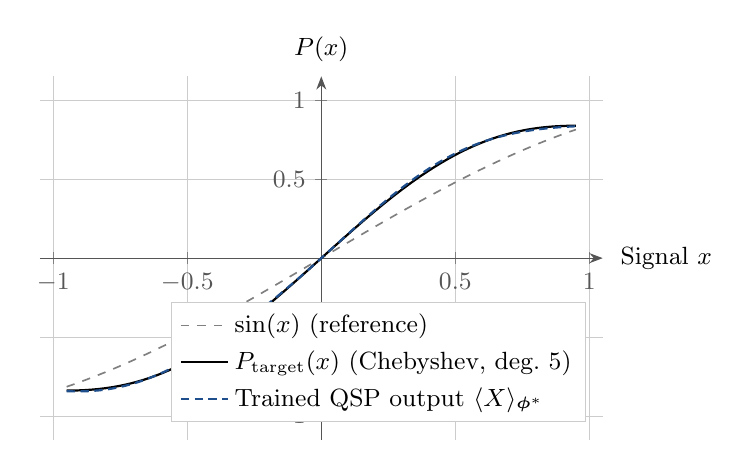
\begin{tikzpicture}
\begin{axis}[
  width=0.72\textwidth, height=6.2cm,
  xlabel={Signal $x$},
  ylabel={$P(x)$},
  xmin=-1.05, xmax=1.05,
  ymin=-1.15, ymax=1.15,
  xtick={-1,-0.5,0,0.5,1},
  ytick={-1,-0.5,0,0.5,1},
  grid=both,
  grid style={line width=0.3pt, draw=lightrule},
  axis lines=center,
  axis line style={-Stealth, thin, graytext},
  xlabel style={font=\small, at={(axis cs:1.08,0)}, anchor=west},
  ylabel style={font=\small, at={(axis cs:0,1.18)}, anchor=south},
  tick label style={font=\small, color=graytext},
  legend style={font=\small, at={(0.97,0.05)}, anchor=south east,
                draw=lightrule, fill=white, row sep=1pt},
  legend cell align=left,
]
\addplot[gray, dashed, semithick, domain=-0.95:0.95, samples=80]
  {sin(deg(x))};
\addlegendentry{$\sin(x)$ (reference)}

\addplot[black, thick, domain=-0.95:0.95, samples=80]
  {1.5257*x - 0.9416*x^3 + 0.2528*x^5};
\addlegendentry{$P_{\mathrm{target}}(x)$ (Chebyshev, deg.\ 5)}

\addplot[accent, thick, densely dashed, domain=-0.95:0.95, samples=80]
  {1.5257*x - 0.9416*x^3 + 0.2528*x^5 + 0.04*sin(deg(5*x))*x*(1-x*x)};
\addlegendentry{Trained QSP output $\langle X\rangle_{\boldsymbol{\phi}^*}$}
\end{axis}
\end{tikzpicture}
\caption{Polynomial approximation quality. The trained QSP circuit (blue, dashed) closely tracks the degree-5 Chebyshev target $P_{\mathrm{target}}$ (black). The residual gap between $P_{\mathrm{target}}$ and the true $\sin(x)$ (grey, dashed) reflects the inherent degree-5 truncation error, not a limitation of the gradient learning procedure.}
\label{fig:poly}
\end{figure}

%% ============================================================
\section{Discussion}
%% ============================================================

\subsection{Analytic Solvers vs.\ Gradient Training}

\begin{table}[ht]
\centering\small
\begin{tabularx}{\textwidth}{@{} X l @{}}
  \toprule
  \textbf{Scenario} & \textbf{Recommended approach} \\
  \midrule
  Known target polynomial, degree $<10^3$       & Analytic solver \\
  Implicit loss (e.g.\ energy minimization)      & Gradient training \\
  QSP as subroutine in a larger VQA              & End-to-end gradient training \\
  Degree $>10^3$                                 & Iterative analytic solver~\cite{chao2020finding} \\
  Novel polynomial with no closed form           & Gradient training \\
  \bottomrule
\end{tabularx}
\caption{Decision guide: when to use analytic angle computation vs.\ gradient-based learning.}
\label{tab:decision}
\end{table}

\subsection{Loss Landscape and Scaling}

The QSP loss landscape is non-convex. At degree~5, a single random seed with small initialization ($|\phi_i|\le0.5$) was sufficient for convergence. Higher degrees ($d\gg10$) are expected to produce a more complex landscape with more local minima, potentially requiring curriculum learning over degree, better initialization, or second-order methods.

\subsection{The JAX Traceability Constraint}

The flat-circuit pattern described in Section~3.3 is the correct workaround for JAX-based variational optimization of QSP circuits, and is expected to generalize to multi-qubit block-encoding extensions and to other quantum SDKs when the same traceability rules are respected. JAX transforms functions by tracing them with abstract values; any component that captures concrete arrays at construction time exits the trace. This is not unique to PennyLane---it is a general pitfall for template-heavy circuit APIs combined with JAX-style AD.

\subsection{Reproducibility}

The full implementation is publicly available under Apache~2.0 at \url{https://github.com/rosspeili/trainable-qsp-angles}~\cite{peili_trainable_qsp_2026}. An interactive Jupyter notebook (\texttt{demo.ipynb}) is included in the repository.

%% ============================================================
\section{Food for Thought}
%% ============================================================

Quantum Signal Processing is, at its core, a statement about \emph{expressibility}: any bounded-parity polynomial can be realized by a structured single-qubit circuit. This is a completeness result --- not merely an existence proof, but a constructive recipe. What the gradient approach adds is a \emph{learning} recipe: given any differentiable objective, one can search the space of realizable polynomials by moving through the space of phase angles.

\textbf{What is a quantum algorithm, really?} The grand unification perspective of~\cite{martyn2021grand} suggests that many quantum algorithms are the same circuit architecture differentiated only by their phase angle sequence. If phase angles can be \emph{learned} rather than derived, the boundary between algorithm design and machine learning in the quantum domain becomes blurry. Are we designing algorithms, or training them?

This is not merely philosophical. In the classical world, the success of deep learning has demonstrated that learned programs can solve problems for which no analytic solution is known, often by discovering structure the algorithm designer did not anticipate. QSP provides a quantum analogue: a parameterized circuit with a clear mathematical interpretation of what its parameters control. Unlike generic variational circuits (expressive but opaque), QSP circuits are \emph{interpretable} --- each phase sequence corresponds to a specific polynomial with a direct operational meaning.

The gradient-trained QSP circuit is therefore a peculiar object: simultaneously a machine-learned artifact (its parameters were found by optimization) and a provably structured quantum program (its output is a bounded polynomial in the signal). This combination --- optimization within a mathematically transparent space --- may be a productive template for the broader challenge of quantum algorithm discovery.

One further provocation: the NISQ era~\cite{preskill2018quantum} has been characterized by variational algorithms that optimize generic parameterized circuits for heuristic objectives. QSP offers an alternative: variational circuits that are not generic, but \emph{complete within a well-defined polynomial class}. The question is whether that polynomial class is expressive enough for practically relevant tasks beyond quantum simulation. We believe the answer is likely yes --- and that gradient-based QSP learning is one of the more principled paths toward finding out.

%% ============================================================








\nocite{*}
\printbibliography



\end{document}
